\section{Module und Pakete}

\begin{frame}[fragile]
\frametitle{Module importieren}
Funktionen, Klassen und Objekte, die thematisch zusammengeh"oren, werden in Modulen geb"undelt.
\begin{lstlisting}[style=Python]
import math
s = math.sin(math.pi)
\end{lstlisting}
\begin{lstlisting}[style=Python]
import math as m
s = m.sin(m.pi)
\end{lstlisting}
\begin{lstlisting}[style=Python]
from math import pi as PI, sin
s = sin(PI)
\end{lstlisting}
\begin{lstlisting}[style=Python]
from math import *
s = sin(pi)
\end{lstlisting}
\end{frame}

\begin{frame}[fragile]
\frametitle{Module}
\begin{itemize}
\item Hilfe: \lstinline{dir(math)}, \lstinline{help(math)}
\item Module werden gesucht in:
\begin{itemize}
\item dem Verzeichnis der aufrufenden Datei
\item Verzeichnissen aus der Umgebungsvariablen \texttt{PYTHONPATH}
\item installationsbedingten Verzeichnissen 
\end{itemize}
\end{itemize}
\begin{lstlisting}[style=Shell]
>>> import sys
>>> sys.path
['', '/usr/lib/python24.zip',
 '/usr/lib/python2.4', 
 '/usr/lib/python2.4/site-packages', ...]
\end{lstlisting}
\end{frame}

\begin{frame}[fragile]
\frametitle{Pakete importieren}
Module k"onnen zu  hierarchisch strukturierten Paketen zusammengefasst werden.
\begin{lstlisting}[style=Python]
from email.mime import text as mtext
msg = mtext.MIMEText("Hallo Welt!")
\end{lstlisting}
\begin{lstlisting}[style=Python]
from email.mime.text import MIMEText
msg = MIMEText("Hallo Welt!")
\end{lstlisting}
\end{frame}

\begin{frame}[fragile]
\frametitle{Eigene Module}
Jedes Python-Programm kann als Modul importiert werden.
\begin{lstlisting}[style=Python]
"""Mein erstes Modul: mein_modul.py"""

def add(a, b):
   """Addiere a und b."""
   return a + b

print add(2, 3)
\end{lstlisting}
\begin{lstlisting}[style=Shell]
>>> import mein_modul
5
>>> mein_modul.add(17, 42)
59
\end{lstlisting}
Top-Level-Anweisungen werden beim Import ausgef"uhrt!
\end{frame}

\begin{frame}[fragile]
Sollen Anweisungen nur beim direkten Ausf"uhren, nicht beim Importieren ausgef"uhrt werden:
\frametitle{Eigene Module}
\vspace{3mm}
\begin{lstlisting}[style=Python]
def add(a, b):
   return a + b

def main():
    print add(2, 3)

if __name__ == "__main__":
    main()
\end{lstlisting}
Sinnvoll z.B. f"ur Tests.
\end{frame}

\begin{frame}[fragile]
\frametitle{Eigene Pakete}
\begin{columns}
\begin{column}{3.2cm}
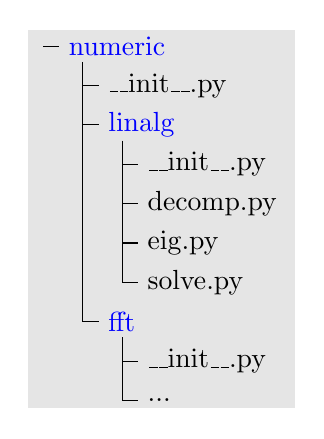
\begin{tikzpicture}
\fill[black!10!white] (-0.2,  0.2) rectangle (3.2, -4.6);
\draw (0.0,  0.0) -- (0.2,  0.0) node[anchor=west] {\color{blue}numeric};
\draw (0.5, -0.2) -- (0.5, -3.5);
\draw (0.5, -0.5) -- (0.7, -0.5) node[anchor=west] {\_\_init\_\_.py};
\draw (0.5, -1.0) -- (0.7, -1.0) node[anchor=west] {\color{blue}linalg};
\draw (1.0, -1.2) -- (1.0, -3.0);
\draw (1.0, -1.5) -- (1.2, -1.5) node[anchor=west] {\_\_init\_\_.py};
\draw (1.0, -2.0) -- (1.2, -2.0) node[anchor=west] {decomp.py};
\draw (1.0, -2.5) -- (1.2, -2.5) node[anchor=west] {eig.py};
\draw (1.0, -3.0) -- (1.2, -3.0) node[anchor=west] {solve.py};
\draw (0.5, -3.5) -- (0.7, -3.5) node[anchor=west] {\color{blue}fft};
\draw (1.0, -3.7) -- (1.0, -4.5);
\draw (1.0, -4.0) -- (1.2, -4.0) node[anchor=west] {\_\_init\_\_.py};
\draw (1.0, -4.5) -- (1.2, -4.5) node[anchor=west] {...};
\end{tikzpicture}
\end{column}
\begin{column}{7.3cm}
In jedem Paket-Ordner: \lstinline{__init__.py} \\
(kann leer sein)
\vspace{2mm}
\begin{lstlisting}[style=Python]
import numeric
numeric.foo() #Aus __init__.py
numeric.linalg.eig.foo()
\end{lstlisting}
\begin{lstlisting}[style=Python]
from numeric.linalg import eig
eig.foo()
\end{lstlisting}
\end{column}
\end{columns}
\end{frame}

%%% Local Variables: 
%%% mode: latex
%%% latex-run-command: pdflatex
%%% TeX-master: "vortrag"
%%% End: 
